
\فصل{مفاهیم اولیه}

% stroke types
% aspects
% thrombectomy
% aspect slices
% ct and dicom

% segmentation
% augmentation
% transfer learning
% pretrained models
% cross validation

در این فصل به ذکر برخی مفاهیم اولیه‌ی مورد ارجاع در ادامه‌ی پایان‌نامه پرداخته می‌شود.
این مفاهیم در دو دسته‌ی پزشکی و فنی قابل بررسی هستند.
در ابتدا، مبانی پزشکی موضوع پروژه و نکاتی حول تصاویر پزشکی مورد استفاده به اختصار شرح داده می‌شود.
در ادامه نیز نکاتی در رابطه با هسته‌ی فنی پروژه و روش‌های مورد استفاده در یادگیری ماشین ذکر می‌گردد.
به این ترتیب، این فصل می‌تواند در دست‌یابی به یک دانش مشترک در میان متخصصان هر دو حوزه اثربخش باشد.

\قسمت{مفاهیم پزشکی}

\زیرقسمت{سکته‌ی مغزی}

انواع سکته‌های مغزی شامل دو دسته‌ی کلی سکته‌های انسدادی
\footnote{ischemic}
و خونریزی
\footnote{haemorrhagic} 
هستند.
سکته‌ی مغزی انسدادی به علت قطع شدن جریان خون به بخشی از مغز رخ می‌دهد که باعث از دست رفتن ناگهانی عملکرد آن ناحیه می‌شود.
در مقابل، سکته‌ی مغزی خونریزی از پاره‌شدن یک رگ خونی و یا ساختار غیر طبیعی عروقی نشأت می‌گیرد.
در یک نگاه کلی، تقریبا ۸۰٪ بیماران سکته‌ی مغزی، در دسته‌ی اول، یعنی سکته‌ی انسدادی، قرار می‌گیرند.
%https://www.ncbi.nlm.nih.gov/pmc/articles/PMC6288566/ Stroke in the 21st Century: A Snapshot of the Burden, Epidemiology, and Quality of Life
این دو نوع سکته‌ی مغزی، ظاهر متفاوتی در تصاویر CT به خود می‌گیرند.
تصویر ~\ref{fig:ischemic-harmorhagic} این تفاوت را نشان می‌دهد.
همانطور که در این تصویر نمایان است، عموما تشخیص ناحیه‌ی درگیری
در سکته‌ی خونریزی ساده‌تر است و در مقابل، تشخیص این نواحی در سکته‌ی انسدادی، ظرافت و دقت بیشتری نیاز دارد.
همانطور که در تعریف امتیاز ASPECT خواهد آمد، عنوان پژوهش حاضر نیز، زیرمجموعه‌ی 
سکته‌های انسدادی قرار می‌گیرد و تمام مفاهیم مورد اشاره در این پایان‌نامه و تمام تصاویر مورد استفاده نیز به این نوع سکته اشاره خواهند داشت.

\begin{figure}[ht]
\centering
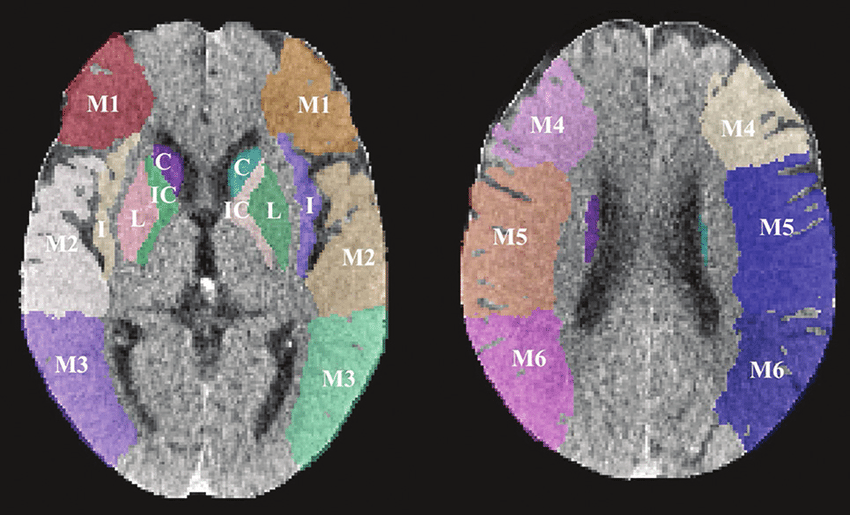
\includegraphics[width=\textwidth, keepaspectratio]{aspects-regions.png}
\caption[]{انواع سکته‌ی مغزی در تصاویر ،CT برش مغزی A یک نمونه سکته‌ی انسدادی و برش B یک نمونه از سکته‌ی خونریزی در این تصاویر را نشان می‌دهد.}
\label{fig:ischemic-haemorrhagic}
\end{figure}
%Ischemic and hemorrhagic brain injury during venoarterial-extracorporeal membrane oxygenation
        

% \begin{figure}[ht]
% \centering
% 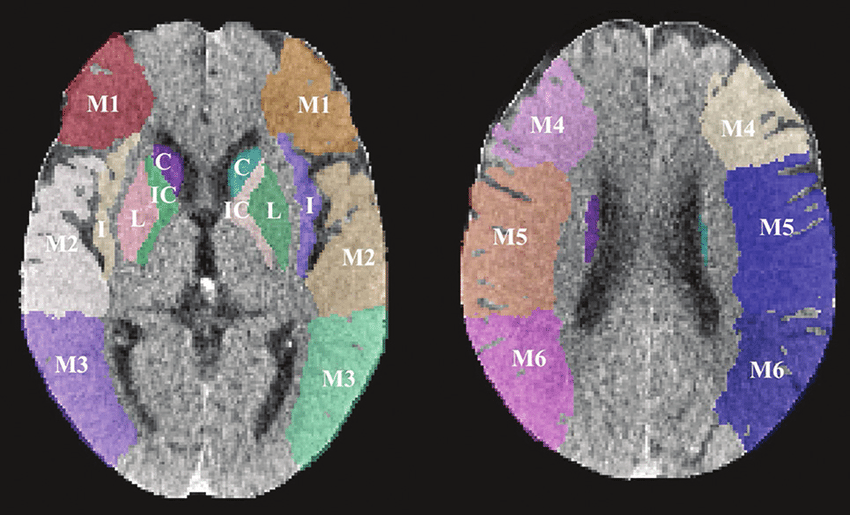
\includegraphics[width=\textwidth, keepaspectratio]{aspects-regions.png}
% \caption[]{نواحی ASPECTS در دو برش از مغز. ۱۰ ناحیه شامل ،I ،C ،L ،IC \lr{M6}-\lr{M1}.}
% \label{fig:aspects-regions}
% \end{figure}
% %Kuang, Hulin & Najm, Mohamed & Chakraborty, Debabrata & Maraj, Nicholas & Sohn, Sung-Il & Goyal, Mayank & Hill, Michael & Demchuk, Andrew & Menon, Bijoy & Qiu, Wu. (2018). Automated ASPECTS on Non-Contrast CT Scans in Acute Ischemic Stroke Patients Using Machine Learning. American Journal of Neuroradiology. 10.3174/ajnr.A5889. 

    
پرونده‌ی اصلی پایان‌نامه در قالب استاندارد\زیرنویس{
قالب استاندارد از گیت‌هاب به نشانی
\href{https://github.com/zarrabi/thesis-template}
{github.com/zarrabi/thesis-template}
قابل دریافت است.}
\کد{thesis.tex}  نام دارد.
به ازای هر فصل از پایان‌نامه، یک پرونده در شاخه‌ی \کد{chapters} ایجاد نموده
و نام آن را در  \کد{thesis.tex} (در قسمت فصل‌ها) درج نمایید.
برای مشاهده‌ی خروجی، پرونده‌ی \کد{thesis.tex} را با زی‌لاتک کامپایل کنید.
مشخصات اصلی پایان‌نامه را می‌توانید در پرونده‌ی \کد{front/info.tex} ویرایش کنید.

\زیرقسمت{عبارات ریاضی}

برای درج عبارات ریاضی در داخل متن از \$...\$ و 
برای درج عبارات ریاضی در یک خط مجزا از \$\$...\$\$ یا محیط \لر{equation} 
استفاده کنید. برای مثال عبارت 
$2x + 3y$
در داخل متن و عبارت زیر
\begin{equation}
\sum_{k=0}^{n} {n \choose k} = 2^n
\end{equation}
در یک خط مجزا درج شده است. 
دقت کنید که تمامی عبارات ریاضی، از جمله متغیرهای تک‌حرفی مانند $x$ و $y$ باید در محیط ریاضی 
یعنی محصور بین دو علامت \$ باشند. 


\زیرقسمت{علائم ریاضی پرکاربرد}

برخی علائم ریاضی پرکاربرد در زیر فهرست شده‌اند. 
برای مشاهده‌ی دستور  معادل پرونده‌ی منبع را ببینید.


\شروع{فقرات}
\فقره مجموعه‌‌های اعداد: 
$\IN, \IZ, \IZ^+, \IQ, \IR, \IC$
\فقره مجموعه:
$\set{1, 2, 3}$
\فقره دنباله‌:
$\seq{1, 2, 3}$
\فقره سقف و کف:
$\ceil{x}, \floor{x}$
\فقره اندازه و متمم:
$\card{A}, \setcomp{A}$
\فقره همنهشتی:
$a \iequiv{n} 1$
یا
$a \equiv 1 \imod{n}$ 
%\فقره شمردن (عاد کردن):
%$3 \divs n, 2 \ndivs n$
\فقره ضرب و تقسیم:
$\times, \cdot, \div$
\فقره سه‌نقطه‌:
$1, 2, \dots, n$
\فقره کسر و ترکیب:
${n \over k}, {n \choose k}$
\فقره اجتماع و اشتراک:
$A \cup (B \cap C)$
\فقره عملگرهای منطقی:
$\neg p \vee (q \wedge r)$

\فقره پیکان‌ها:
$\rightarrow, \Rightarrow, \leftarrow, \Leftarrow, \leftrightarrow, \Leftrightarrow$
\فقره عملگرهای مقایسه‌ای:
$\not=, \le, \not\le, \ge, \not\ge$
\فقره عملگرهای مجموعه‌ای:
$\in, \not\in, \setminus, \subset, \subseteq, \subsetneq, \supset, \supseteq, \supsetneq$

\فقره جمع و ضرب چندتایی:
$\sum_{i=1}^{n} a_i, \prod_{i=1}^{n} a_i$
\فقره اجتماع و اشتراک چندتایی:
$\bigcup_{i=1}^{n} A_i, \bigcap_{i=1}^{n} A_i$
\فقره برخی نمادها:
$\infty, \emptyset, \forall, \exists, \triangle, \angle, \ell, \equiv, \therefore$
\پایان{فقرات}


\زیرقسمت{لیست‌ها}

برای ایجاد یک لیست‌ می‌توانید از محیط‌های «فقرات» و «شمارش» همانند زیر استفاده کنید.

\begin{multicols}{2}
\شروع{فقرات}
\فقره مورد اول
\فقره مورد دوم
\فقره مورد سوم
\پایان{فقرات}

\شروع{شمارش}
\فقره مورد اول
\فقره مورد دوم
\فقره مورد سوم
\پایان{شمارش}

\end{multicols}


\زیرقسمت{درج شکل}

یکی از روش‌های مناسب برای ایجاد شکل استفاده از نرم‌افزار \لر{LaTeX Draw} و سپس
درج خروجی آن به صورت یک فایل \کد{tex} درون متن 
با استفاده از دستور  \کد{fig} یا \کد{centerfig} است.
شکل~\رجوع{شکل:پوشش رأسی} نمونه‌ای از اشکال ایجادشده با این ابزار را نشان می‌دهد.


\شروع{شکل}[ht]
\centerfig{cover.tex}{.9}
\شرح{یک گراف و پوشش رأسی آن}
\برچسب{شکل:پوشش رأسی}
\پایان{شکل}

\bigskip
همچنین می‌توانید با استفاده از نرم‌افزار \lr{Ipe} شکل‌های خود را مستقیما
به صورت \لر{pdf} ایجاد نموده و آن‌ها را با دستورات \کد{img} یا  \کد{centerimg} 
درون متن درج کنید. برای نمونه، شکل~\رجوع{شکل:گراف جهت‌دار} را ببینید.


\شروع{شکل}[ht]
\centerimg{strip}{6.5cm}
\شرح{نمونه شکل ایجادشده توسط نرم‌افزار \lr{Ipe}}
\برچسب{شکل:گراف جهت‌دار}
\پایان{شکل}


\زیرقسمت{درج جدول}

برای درج جدول می‌توانید با استفاده از دستور  «جدول»
جدول را ایجاد کرده و سپس با دستور  «لوح»  آن را درون متن درج کنید.
برای نمونه جدول~\رجوع{جدول:عملگرهای مقایسه‌ای} را ببینید.

\vspace{1.5em}

\شروع{لوح}[ht]
\تنظیم‌ازوسط
\شرح{عملگرهای مقایسه‌ای}

\شروع{جدول}{|c|c|}
\خط‌پر 
\سیاه عملگر & \سیاه عنوان \\ 
\خط‌پر \خط‌پر 
\کد{<} & کوچک‌تر \\ 
\کد{>} & بزرگ‌تر \\
\کد{==} &  مساوی \\ 
\کد{<>} & نامساوی \\ 
\خط‌پر
\پایان{جدول}

\برچسب{جدول:عملگرهای مقایسه‌ای}
\پایان{لوح}



\زیرقسمت{درج الگوریتم}

برای درج الگوریتم می‌توانید از محیط «الگوریتم» استفاده کنید.
یک نمونه در الگوریتم~\رجوع{الگوریتم: پوشش رأسی حریصانه} آمده است.

\شروع{الگوریتم}{پوشش رأسی حریصانه}
\ورودی گراف $G=(V, E)$
\خروجی یک پوشش رأسی از $G$

\دستور قرار بده $C = \emptyset$  % \توضیحات{مقداردهی اولیه}
\تاوقتی{$E$ تهی نیست}
%\اگر{$|E| > 0$}
%	\دستور{یک کاری انجام بده}
%\پایان‌اگر
\دستور یال دل‌‌خواه $uv \in E$ را انتخاب کن
\دستور رأس‌های $u$ و $v$ را به $C$ اضافه کن
\دستور تمام یال‌های واقع بر $u$ یا $v$ را از $E$ حذف کن
\پایان‌تاوقتی
\دستور $C$ را برگردان
\پایان{الگوریتم}


\زیرقسمت{محیط‌های ویژه}

برای درج مثال‌ها، قضیه‌ها، لم‌ها و نتیجه‌ها به ترتیب از محیط‌های
«مثال»، «قضیه»، «لم» و «نتیجه» استفاده کنید.
برای درج اثبات قضیه‌ها و لم‌ها  از محیط «اثبات» استفاده کنید.

تعریف‌های داخل متن را با استفاده از دستور «مهم» به صورت \مهم{تیره‌} نشان دهید.
تعریف‌های پایه‌ای‌تر را درون محیط «تعریف» قرار دهید.

\شروع{تعریف}[اصل لانه‌کبوتری]
اگر $n+1$ کبوتر یا بیش‌تر درون  $n$ لانه قرار گیرند، آن‌گاه لانه‌ای 
وجود دارد که شامل حداقل دو کبوتر است.
\پایان{تعریف}




\قسمت{برخی نکات نگارشی}

این فصل حاوی برخی نکات ابتدایی ولی بسیار مهم در نگارش متون فارسی است. 
نکات گردآوری‌شده در این فصل به‌ هیچ‌ وجه کامل نیست، 
ولی دربردارنده‌ی حداقل مواردی است که رعایت آن‌ها در نگارش پایان‌نامه ضروری به نظر می‌رسد.

\زیرقسمت{فاصله‌گذاری}

\شروع{شمارش}

\فقره 
علائم سجاوندی مانند نقطه، ویرگول، دونقطه، نقطه‌ویرگول، علامت سؤال و علامت تعجب % (. ، : ؛ ؟ !) 
بدون فاصله از کلمه‌ی پیشین خود نوشته می‌شوند، ولی بعد از آن‌ها باید یک فاصله‌ قرار گیرد. مانند: من، تو، او.
\فقره 
علامت‌های پرانتز، آکولاد، کروشه، نقل قول و نظایر آن‌ها بدون فاصله با عبارات داخل خود نوشته می‌شوند، ولی با عبارات اطراف خود یک فاصله دارند. مانند: (این عبارت) یا \{آن عبارت\}.
\فقره 
دو کلمه‌ی متوالی در یک جمله همواره با یک فاصله از هم جدا می‌شوند، ولی اجزای یک کلمه‌ی مرکب باید با نیم‌فاصله\زیرنویس{«نیم‌فاصله» فاصله‌‌ای مجازی است که در عین جدا کردن اجزای یک کلمه‌ی مرکب از یک‌دیگر، آن‌ها را نزدیک به هم نگه می‌دارد. معمولاً برای تولید این نوع فاصله در صفحه‌کلید‌های استاندارد از ترکیب Shift+Space استفاده می‌شود.}‌‌
 از هم جدا شوند. مانند: کتاب درس، محبت‌آمیز، دوبخشی.
 \فقره 
 اجزای فعل‌های مرکب با فاصله از یک‌دیگر نوشته می‌شوند، مانند: تحریر کردن، به سر آمدن.
\پایان{شمارش}


\زیرقسمت{شکل حروف}

\شروع{شمارش}

\فقره 
در متون فارسی به جای حروف «ك» و «ي» عربی باید از حروف «ک» و «ی» فارسی استفاده شود. همچنین به جای اعداد عربی مانند ٥ و ٦ باید از اعداد فارسی مانند ۵ و ۶ استفاده نمود. 
برای این کار، توصیه می‌شود صفحه‌کلید‌ فارسی استاندارد\زیرنویس{\href{http://persian-computing.ir/download/Iranian_Standard_Persian_Keyboard_(ISIRI_9147)_(Version_2.0).zip}{صفحه‌کلید فارسی استاندارد برای ویندوز}، تهیه‌شده توسط بهنام اسفهبد} را بر روی سیستم خود نصب کنید.
\فقره 
عبارات نقل‌قول‌شده یا مؤکد باید درون علامت نقل قولِ «» قرار گیرند، نه ''``. مانند: «کشور ایران».
\فقره 
کسره‌ی اضافه‌ی بعد از «ه» غیرملفوظ به صورت «ه‌ی» یا «هٔ» نوشته می‌شود. مانند: خانه‌ی علی، دنباله‌ی فیبوناچی.

        تبصره‌: اگر «ه» ملفوظ باشد، نیاز به «‌ی» ندارد. مانند: فرمانده دلیر، پادشه خوبان. 

\فقره 
پایه‌های همزه در کلمات، همیشه «ئـ» است، مانند: مسئله و مسئول، مگر در مواردی که همزه ساکن است که در این ‌صورت باید متناسب با اعراب حرف پیش از خود نوشته شود. مانند: رأس، مؤمن. 

\پایان{شمارش}


\زیرقسمت{جدانویسی}

\شروع{شمارش}


\فقره 
علامت استمرار، «می»، توسط نیم‌فاصله از جزء‌ بعدی فعل جدا می‌شود. مانند: می‌رود، می‌توانیم.
\فقره 
شناسه‌های «ام»، «ای»، «ایم»، «اید» و «اند» توسط نیم‌فاصله، و شناسه‌ی «است» توسط فاصله از کلمه‌ی پیش از خود جدا می‌شوند. مانند: گفته‌ام، گفته‌ای، گفته است.
\فقره 
علامت جمع «ها» توسط نیم‌فاصله از کلمه‌ی پیش از خود جدا می‌شود. مانند: این‌ها، کتاب‌ها.
\فقره 
«به» همیشه جدا از کلمه‌ی بعد از خود نوشته می‌شود، مانند: به‌ نام و به آن‌ها، مگر در مواردی که «بـ» صفت یا فعل ساخته است. مانند: بسزا، ببینم.
\فقره 
«به» همواره با فاصله از کلمه‌ی بعد از خود نوشته می‌شود، مگر در مواردی که «به» جزئی از یک اسم یا صفت مرکب است. مانند: تناظر یک‌به‌یک، سفر به تاریخ. 
%\پایان{شمارش}
%
%
%\زیرقسمت{جدانویسی مرجح}
%
%\شروع{شمارش}

%\فقره 
%اجزای اسم‌ها، صفت‌ها، و قیدهای مرکب توسط نیم‌فاصله از یک‌دیگر جدا می‌شوند. مانند: دانش‌جو، کتاب‌خانه، گفت‌وگو، آن‌گاه، دل‌پذیر.
%
%        تبصره: اجزای منتهی به «هاء ملفوظ» را می‌توان از این قانون مستثنی کرد. مانند: راهنما، رهبر. 

\فقره 
علامت صفت برتری، «تر»، و علامت صفت برترین، «ترین»، توسط نیم‌فاصله از کلمه‌ی پیش از خود جدا می‌شوند. 
مانند: سنگین‌تر، مهم‌ترین.

        تبصره‌: کلمات «بهتر» و «بهترین» را می‌توان از این قاعده مستثنی نمود. 

\فقره 
پیشوندها و پسوندهای جامد، چسبیده به کلمه‌ی پیش یا پس از خود نوشته می‌شوند. مانند: همسر، دانشکده، دانشگاه.

        تبصره‌: در مواردی که خواندن کلمه دچار اشکال می‌شود، می‌توان پسوند یا پیشوند را جدا کرد. مانند: هم‌میهن، هم‌ارزی. 

\فقره 
ضمیرهای متصل چسبیده به کلمه‌ی پیش‌ از خود نوشته می‌شوند. مانند: کتابم، نامت، کلامشان. 

\پایان{شمارش}

